\documentclass[12pt,twoside]{article}
\usepackage[dvipsnames]{xcolor}
\usepackage{tikz,graphicx,amsmath,amsfonts,amscd,amssymb,bm,cite,epsfig,epsf,url}
\usepackage[hang,flushmargin]{footmisc}
\usepackage[colorlinks=true,urlcolor=blue,citecolor=blue]{hyperref}
\usepackage{amsthm,multirow,wasysym,appendix}
\usepackage{array,subcaption} 
% \usepackage[small,bf]{caption}
\usepackage{bbm}
\usepackage{pgfplots}
\usetikzlibrary{spy}
\usepgfplotslibrary{external}
\usepgfplotslibrary{fillbetween}
\usetikzlibrary{arrows,automata}
\usepackage{thmtools}
\usepackage{blkarray} 
\usepackage{textcomp}
\usepackage[left=0.8in,right=1.0in,top=1.0in,bottom=1.0in]{geometry}

%% Probability operators and functions
%
% \def \P{\mathrm{P}}
\def \P{\mathrm{P}}
\def \E{\mathrm{E}}
\def \Var{\mathrm{Var}}
\let\var\Var
\def \Cov {\mathrm{Cov}} \let\cov\Cov
\def \MSE {\mathrm{MSE}} \let\mse\MSE
\def \sgn {\mathrm{sgn}}
\def \R {\mathbb{R}}
\def \C {\mathbb{C}}
\def \N {\mathbb{N}}
\def \Z {\mathbb{Z}}
\def \cV {\mathcal{V}}
\def \cS {\mathcal{S}}

\newcommand{\RR}{\ensuremath{\mathbb{R}}}

\DeclareMathOperator*{\argmin}{arg\,min}
\DeclareMathOperator*{\argmax}{arg\,max}
\newcommand{\red}[1]{\textcolor{red}{#1}}
\newcommand{\blue}[1]{\textcolor{blue}{#1}}
\newcommand{\green}[1]{\textcolor{ForestGreen}{ #1}}
\newcommand{\fuchsia}[1]{\textcolor{RoyalPurple}{ #1}}



%
%% Probability distributions
%
%\def \Bern    {\mathrm{Bern}}
%\def \Binom   {\mathrm{Binom}}
%\def \Exp     {\mathrm{Exp}}
%\def \Geom    {\mathrm{Geom}}
% \def \Norm    {\mathcal{N}}
%\def \Poisson {\mathrm{Poisson}}
%\def \Unif    {\mathrm {U}}
%
\DeclareMathOperator{\Norm}{\mathcal{N}}

\newcommand{\bdb}[1]{\textcolor{red}{#1}}

\newcommand{\ml}[1]{\mathcal{ #1 } }
\newcommand{\wh}[1]{\widehat{ #1 } }
\newcommand{\wt}[1]{\widetilde{ #1 } }
\newcommand{\conj}[1]{\overline{ #1 } }
\newcommand{\rnd}[1]{\tilde{ #1 } }
\newcommand{\rv}[1]{ \rnd{ #1}  }
\newcommand{\rM}{\rnd{ m}  }
\newcommand{\rx}{\rnd{ x}  }
\newcommand{\ry}{\rnd{ y}  }
\newcommand{\rz}{\rnd{ z}  }
\newcommand{\ra}{\rnd{ a}  }
\newcommand{\rb}{\rnd{ b}  }
\newcommand{\rt}{\rnd{ t}  }
\newcommand{\rs}{\rnd{ s}  }


\newcommand{\rpc}{\widetilde{ pc}  }
\newcommand{\rndvec}[1]{\vec{\rnd{#1}}}

\def \cnd {\, | \,}
\def \Id { I }
\def \J {\mathbf{1}\mathbf{1}^T}

\newcommand{\op}[1]{\operatorname{#1}}
\newcommand{\setdef}[2]{ := \keys{ #1 \; | \; #2 } }
\newcommand{\set}[2]{ \keys{ #1 \; | \; #2 } }
\newcommand{\sign}[1]{\op{sign}\left( #1 \right) }
\newcommand{\trace}[1]{\op{tr}\left( #1 \right) }
\newcommand{\tr}[1]{\op{tr}\left( #1 \right) }
\newcommand{\inv}[1]{\left( #1 \right)^{-1} }
\newcommand{\abs}[1]{\left| #1 \right|}
\newcommand{\sabs}[1]{| #1 |}
\newcommand{\keys}[1]{\left\{ #1 \right\}}
\newcommand{\sqbr}[1]{\left[ #1 \right]}
\newcommand{\sbrac}[1]{ ( #1 ) }
\newcommand{\brac}[1]{\left( #1 \right) }
\newcommand{\bbrac}[1]{\big( #1 \big) }
\newcommand{\Bbrac}[1]{\Big( #1 \Big)}
\newcommand{\BBbrac}[1]{\BIG( #1 \Big)}
\newcommand{\MAT}[1]{\begin{bmatrix} #1 \end{bmatrix}}
\newcommand{\sMAT}[1]{\left(\begin{smallmatrix} #1 \end{smallmatrix}\right)}
\newcommand{\sMATn}[1]{\begin{smallmatrix} #1 \end{smallmatrix}}
\newcommand{\PROD}[2]{\left \langle #1, #2\right \rangle}
\newcommand{\PRODs}[2]{\langle #1, #2 \rangle}
\newcommand{\der}[2]{\frac{\text{d}#2}{\text{d}#1}}
\newcommand{\pder}[2]{\frac{\partial#2}{\partial#1}}
\newcommand{\derTwo}[2]{\frac{\text{d}^2#2}{\text{d}#1^2}}
\newcommand{\ceil}[1]{\lceil #1 \rceil}
\newcommand{\Imag}[1]{\op{Im}\brac{ #1 }}
\newcommand{\Real}[1]{\op{Re}\brac{ #1 }}
\newcommand{\norm}[1]{\left|\left| #1 \right|\right| }
\newcommand{\norms}[1]{ \| #1 \|  }
\newcommand{\normProd}[1]{\left|\left| #1 \right|\right| _{\PROD{\cdot}{\cdot}} }
\newcommand{\normTwo}[1]{\left|\left| #1 \right|\right| _{2} }
\newcommand{\normTwos}[1]{ \| #1  \| _{2} }
\newcommand{\normZero}[1]{\left|\left| #1 \right|\right| _{0} }
\newcommand{\normTV}[1]{\left|\left| #1 \right|\right|  _{ \op{TV}  } }% _{\op{c} \ell_1} }
\newcommand{\normOne}[1]{\left|\left| #1 \right|\right| _{1} }
\newcommand{\normOnes}[1]{\| #1 \| _{1} }
\newcommand{\normOneTwo}[1]{\left|\left| #1 \right|\right| _{1,2} }
\newcommand{\normF}[1]{\left|\left| #1 \right|\right| _{\op{F}} }
\newcommand{\normLTwo}[1]{\left|\left| #1 \right|\right| _{\ml{L}_2} }
\newcommand{\normNuc}[1]{\left|\left| #1 \right|\right| _{\ast} }
\newcommand{\normOp}[1]{\left|\left| #1 \right|\right|  }
\newcommand{\normInf}[1]{\left|\left| #1 \right|\right| _{\infty}  }
\newcommand{\proj}[1]{\mathcal{P}_{#1} \, }
\newcommand{\diff}[1]{ \, \text{d}#1 }
\newcommand{\vc}[1]{\boldsymbol{\vec{#1}}}
\newcommand{\rc}[1]{\boldsymbol{#1}}
\newcommand{\vx}{\vec{x}}
\newcommand{\vy}{\vec{y}}
\newcommand{\vz}{\vec{z}}
\newcommand{\vu}{\vec{u}}
\newcommand{\vv}{\vec{v}}
\newcommand{\vb}{\vec{\beta}}
\newcommand{\va}{\vec{\alpha}}
\newcommand{\vaa}{\vec{a}}
\newcommand{\vbb}{\vec{b}}
\newcommand{\vg}{\vec{g}}
\newcommand{\vw}{\vec{w}}
\newcommand{\vh}{\vec{h}}
\newcommand{\vbeta}{\vec{\beta}}
\newcommand{\valpha}{\vec{\alpha}}
\newcommand{\vgamma}{\vec{\gamma}}
\newcommand{\veta}{\vec{\eta}}
\newcommand{\vnu}{\vec{\nu}}
\newcommand{\rw}{\rnd{w}}
\newcommand{\rvnu}{\vc{\nu}}
\newcommand{\rvv}{\rndvec{v}}
\newcommand{\rvw}{\rndvec{w}}
\newcommand{\rvx}{\rndvec{x}}
\newcommand{\rvy}{\rndvec{y}}
\newcommand{\rvz}{\rndvec{z}}
\newcommand{\rvX}{\rndvec{X}}


\newtheorem{theorem}{Theorem}[section]
% \declaretheorem[style=plain,qed=$\square$]{theorem}
\newtheorem{corollary}[theorem]{Corollary}
\newtheorem{definition}[theorem]{Definition}
\newtheorem{lemma}[theorem]{Lemma}
\newtheorem{remark}[theorem]{Remark}
\newtheorem{algorithm}[theorem]{Algorithm}

% \theoremstyle{definition}
%\newtheorem{example}[proof]{Example}
\declaretheorem[style=definition,qed=$\triangle$,sibling=definition]{example}
\declaretheorem[style=definition,qed=$\bigcirc$,sibling=definition]{application}

%
%% Typographic tweaks and miscellaneous
%\newcommand{\sfrac}[2]{\mbox{\small$\displaystyle\frac{#1}{#2}$}}
%\newcommand{\suchthat}{\kern0.1em{:}\kern0.3em}
%\newcommand{\qqquad}{\kern3em}
%\newcommand{\cond}{\,|\,}
%\def\Matlab{\textsc{Matlab}}
%\newcommand{\displayskip}[1]{\abovedisplayskip #1\belowdisplayskip #1}
%\newcommand{\term}[1]{\emph{#1}}
%\renewcommand{\implies}{\;\Rightarrow\;}



\begin{document}

\begin{center}
{\large{\textbf{Homework 3}} } \vspace{0.2cm}\\
Due Feb 12 at 11 pm
\\
\end{center}
Unless stated otherwise, justify any answers you give.
You can work in groups, but each
student must write their own solution based on their own
understanding of the problem.

When uploading your homework to Gradescope you will have to
select the relevant pages for each question.  Please submit each
problem on a separate page (i.e., 1a and~1b can be on the same page but 1
and 2 must be on different pages).  We understand that this may be
cumbersome but this is the best way for the grading team to grade your
homework assignments and provide feedback in a timely manner.  Failure
to adhere to these guidelines may result in a loss of points.
Note that it may take some time to
select the pages for your submission.  Please plan accordingly.  We
suggest uploading your assignment at least 30 minutes before the deadline
so you will have ample time to select the correct pages for your
submission.  If you are using \LaTeX, consider using the minted or
listings packages for typesetting code.  
\\

\begin{enumerate}


\item (Markov's and Chebyshev's inequalities are tight)
In this problem we show that Markov's and Chebyshev's inequalities cannot be improved without further assumptions, because there exist random variables for which they are tight. 
\begin{enumerate}
\item For any $c >0$ and any $0 < \theta < 1$, build a nonnegative random variable $\ra$ such that 
\begin{align}
\P\brac{\ra \geq c} = \theta = \frac{\E\sqbr{ \ra }}{c}.
\end{align} 
\begin{itemize}
    \item the conditions of Markov's inequality are met so we know that $P(\Tilde{a}\geq c)\leq \frac{E[\Tilde{a}]}{c}$
    \item for any $c$ suppose that we define a non-negative random variable $\Tilde{a}$ such that $P(\Tilde{a}\in\{0,c\})=1$ ie $\Tilde{a}$ can only take on values of 0 or c. 
    \item if this is the case we can write $E[\Tilde{a}]=\Sigma_{a\in \mathbb{R}}aP(\Tilde{a}=a)=0P(\Tilde{a}=0)+\Sigma_{a=1}^{c-1}aP(\Tilde{a}=a)+cP(\Tilde{a}=c)\leq 0P(\Tilde{a}=0)+(c)\Sigma_{a=1}^{c-1}P(\Tilde{a}=a)+cP(\Tilde{a}=c)=0+0+P(\Tilde{a}=c)$ further since $\Tilde{a}$ only takes on values c or 0 we know that $P(\Tilde{a}=c)=P(\Tilde{a}\geq c)$ thus we have $E[\Tilde{a}]\leq c P(\Tilde{a}\geq c)\Rightarrow P(\Tilde{a}\geq c) \geq \frac{E[\Tilde{a}]}{c}$ 
    \item so thus we know$  P(\Tilde{a}\geq c) \geq \frac{E[\Tilde{a}]}{c}$ and  $P(\Tilde{a}\geq c) \leq \frac{E[\Tilde{a}]}{c}$ which implies that $ P(\Tilde{a}\geq c) =\frac{E[\Tilde{a}]}{c}$
\end{itemize}

\item For any $c >0$, any $0 < \theta < 1$ and any $\mu \in \R$, build a random variable $\rb$ with mean $\mu$ and finite variance, such that 
\begin{align}
\P\brac{ | \rb - \mu | \geq c} = \theta = \frac{\var\ssqbr{\rb} }{c^2}.
\end{align} 
\begin{itemize}
    \item here we want to build $\Tilde{b}$ such that $(\Tilde{b}-\mu)^2$ satisfy  $P((\Tilde{b}-\mu)^{2}\in \{0,c\})=1$
    \item observe that regardless of the value of $\mu$ if $\Tilde{b}=\sqrt{\mu}$ we have $(\Tilde{b}^{2}-\mu)^2=(\mu-\mu)^2=0$
    \item similarly regardless of the value of $\mu$ if $\Tilde{b}=\sqrt{\mu+c^2}$ then $(\Tilde{b}^{2}-\mu)^2=(c^2+\mu-\mu)^2=c^2$
    \item so if we  design $\Tilde{b}$ such that $P(\Tilde{b}\in \{\mu, c^2+\mu\})=1$ then the random variable $(\Tilde{b}-\mu)^2$ will satisfy our conditions from part one and thus have $P((\Tilde{b}-\mu)^2\geq c)=\frac{E[(\Tilde{b}-\mu)^2]}{c}$
    \item then we can see $P(|\Tilde{b}-\mu|)=P((\Tilde{b}-\mu)^2\geq c^2)= \frac{E[\Tilde{b}-\mu]^2}{c^2}=\frac{var(\Tilde{b})}{c^2}$
\end{itemize}
\end{enumerate}
\newpage
\item (Online poll) In online polls, young people are often overrepresented. In this problem we study how to correct for this. When answering the questions use the following notation: $\alpha$ is the proportion of young people (between 18 and 35 years old) in the population, $\theta_1$ the proportion of young people in the population who will vote for the Democratic candidate, $\theta_2$ the proportion of old people in the population who will vote for the Democratic candidate, $n_1$ the number of young people in the poll, and $n_2$ the number of old people in the poll. Assume that $\alpha$ is known.
\begin{enumerate}
\item Derive an estimator of the proportion of voters that will vote for the Democratic candidate, as a function of the number of young people $y$ and the number of old people $o$ in the poll that intend to vote Democrat. 
\begin{itemize}
    \item we can design an estimator $p=p(o,y)=\alpha(\frac{y}{n_1})+(1-\alpha)(\frac{0}{n_2})$
\end{itemize}
\item Evaluate your estimator for a poll with 100 participants where 60 intend to vote for the Democratic candidate. Out of the 100 participants, 70 are young, and 50 of them intend to vote for the Democratic candidate. The fraction of young people among voters in general is 25\%. 
\begin{itemize}
    \item for a poll with 100 participants where 60 intend to vote for the Democratic candidate our estimator would return a proportion of democrat voters equal to $0.4285714285714286$
\end{itemize}


\item Under what assumptions is your estimator unbiased? Justify your answer mathematically.
\begin{itemize}
    \item we can see that the true proportion of democrat voters in the population is $p_{pop}=\alpha(\theta_1)+(a-\alpha)(\theta_2)$
    \item we can find the expectation of our estimator p as $E[p]=E[\alpha(\frac{y}{n_1})+(1-\alpha)(\frac{0}{n_2})]=E[\alpha(\frac{y}{n_1})]+E[(1-\alpha)(\frac{0}{n_2})]=\frac{\alpha}{n_1}E[y]+\frac{1-\alpha}{n_2}E[o]$
    \item note that we can write $Y=\Sigma_{i=1}{n_1}1(\text{ young person i votes democrat)})$ that is $Y$ (the number of young people in the sample who voted democrat) is the sum of the number of people who chose to vote democrat and
    \item similarly for old people we have $o=\Sigma_{i=1}{n_2}1(\text{ old person i votes democrat)})$
    \item we assume that the young people $y_i$ and old people $o_i$ are sampled IID from respective populations $Y_{pop}, O_{pop}$ and further that the sampling from $Y_{pop}$ is independent of the sampling from $O_{pop}$
    \item if this is the case we can write $y=\Sigma_{i=1}^{n}1(\text{ young person i votes democrat)})=\Sigma_{i=1}{n_1}(y_i)$
    \item thus $E[y]=E[\Sigma_{i=1}{n_1}(y_i)]=(n_1)\Sgima_{i=1}^{n_1}E[y_i]$
    \item as we assumed $y_i$ is iid we know from lecture $E[y_i]=\frac{1}{N}\Sigma_{i=1}^{N}Y_iP(y_i=Y_i)=\theta_1$
    \item thus we have $E[y]=E[\Sigma_{i=1}^{n_1}(y_i)]=(n_1)\Sgima_{i=1}^{n_1}E[y_i]=(n-1)(\theta_1)$
    \item this allows us to write $\frac{E[y]}{n_1}=\frac{\tehta_1 (n_1)}{n_1}=\theta_1$
    \item we can do the same argument for old people to show that under our assumptions $\frac{E[O]}{N_2}=\theta_2$
    \item thus $E[p]=E[\alpha(\frac{y}{n_1})+(1-\alpha)(\frac{0}{n_2})]=E[\alpha(\frac{y}{n_1})]+E[(1-\alpha)(\frac{0}{n_2})]=\frac{\alpha}{n_1}E[y]+\frac{1-\alpha}{n_2}E[o]=\alpha (\tehta_1)+(1-\alpha)\theta_2$
    \item so we can finally see that under our assumptions $p_{pop}-E[p]=\alpha (\tehta_1)+(1-\alpha)\theta_2-\alpha (\tehta_1)+(1-\alpha)\theta_2=0$ and thus $p$ is an unbiased estimator of $p_{pop}$
    \end{itemize}

\item Show that your estimator is consistent as $n_1 \rightarrow \infty$ and  $n_2 \rightarrow \infty$.
\begin{itemize}
    \item we want to show that as $lim_{n_1,n_2\rightarrow \infty}P(|p-p_{pop}|\geq \epsilon=0) $ for any positive $\epsilon$
    \item first we showed that P is unbiased under random sampling assumptions above
    \item now we want to look at the variance of our estimator p.
    \item $var(p)=var(\alpha(\frac{y}{n_1})+(1-\alpha)(\frac{0}{n_2}))$ 
    \item  as we assumed samples are random iid are drawn independently from the young and old populations  $var(p)=var(\alpha(\frac{y}{n_1})+(1-\alpha)(\frac{0}{n_2}))=\frac{\alpha^2}{n_1^2}var(y)+\frac{(1-\alpha)^2}{n_2^2}var(o)$
    \item from here we can say that $var(p)={\alpha^2}var(\frac{y}{n_1})+(1-\alpha)^2var(\frac{o}{n_2})$ 
    \item we can see that $var(\frac{y}{n_1})$ is variance of a sample proportion of an unbiased rv thus $var(\frac{y}{n_1})=var(\frac{1}{n_1}\Sigma_{i=1}^{n_1}\frac{y_i}{n_1}=\frac{1}{n_1^2}\Sigma_{i=1}^{n}var(\frac{y_i}{n-1})=\frac{1}{n_1^{4}}\Sigma_{i=1}^{n}var({y_i})$
    \item $var(y_i)=var((n_1)\Sigma_{i=1}^{n_1}y_i)=n_1^{2}\Sigma_{i=1}^{n}var(y_i)=n_1^{2}\sigma_{y}$ where $\sigma_{y}$ is the population variance of young people. using the fact that $var(y_i)=\Sigma_{i=1}^{N}(Y_{pop_i}-\theta_1)^2P(y_i=Y_{pop_i})=\frac{1}{n}\Sigma_{i=1}^{N}(Y_{pop_i}-\theta_1)^2=\sigma_{y}^2$
    \item so finally we have $var(\frac{y}{n_1})=var(\frac{1}{n_1}\Sigma_{i=1}^{n_1}\frac{y_i}{n_1}=\frac{1}{n_1^2}\Sigma_{i=1}^{n}var(\frac{y_i}{n-1})=\frac{1}{n_1^{4}}\Sigma_{i=1}^{n}var({y_i})=\frac{\sigma_{y}^2}{n_1^2}$
    \item we can repeat the $var(\frac{0}{n_2})=\frac{\sigma_{0}^2}{n_2^2}$
    \item this finally yields that $var(p)=\frac{\alpha^2 \sigma_{y}^2}{n_1^{2}}+\frac{(1-\alpha)^2 \sigma_{o}^2}{n_2^{2}}$
    \item from here we can use Chebyshev's inequality and see that $P(|p-\alpha(\theta_1)+(1-\alpha)(\theta_2)|\geq  \epsilon)\leq \frac{var(p)}{\epsilon^2}=\frac{\alpha\sigma_{y}^2}{n_1^2 \epsilon^2}+\frac{(1-\alpha)\sigma_{o}^2}{n_2^2 \epsilon^2}$
    \item we know that $\epsilon, \alpha$ are fixed thus as $n_1,n_2\rightarrow \infty$ this quantity will approach zero meaning the estimator is consistent 
\end{itemize}


\end{enumerate}
\newpage
\item (Consistency of the sample median) Let $\rx_1$, $\rx_2$, \ldots be a sequence of i.i.d. random variables from a distribution with median $\gamma$. We assume that $\gamma$ is the only point that satisfies $F_{\rx_i}(\gamma) = 1/2$. Let $\widetilde{md}_n$ denote the median of the $n$ first elements of the sequence. In this problem we establish that for any $\epsilon > 0$
\begin{align}
\label{eq:emp_median}
\lim_{n\rightarrow \infty} \P\brac{ \abs{ \widetilde{md}_n - \gamma} \geq  \epsilon} = 0,
\end{align}
so the sample median is a consistent estimator of the median. Specifically, the goal is to prove
\begin{align}
\label{eq:emp_median_geq}
\lim_{n\rightarrow \infty} \P\brac{  \widetilde{md}_n  \geq \gamma + \epsilon} = 0,
\end{align}
because the same argument can be used to prove
\begin{align}
\label{eq:emp_median_leq}
\lim_{n\rightarrow \infty} \P\brac{  \widetilde{md}_n  \leq \gamma - \epsilon} = 0,
\end{align}
and combining \eqref{eq:emp_median_geq} and \eqref{eq:emp_median_leq} yields \eqref{eq:emp_median}.
\begin{enumerate}
\item Let $\rnd{b}$ be the number of elements in $\keys{\rx_1, \ldots, \rx_n}$ greater or equal to $\gamma + \epsilon$. Explain why


\begin{align}
\P\brac{\widetilde{md}_n \geq \gamma + \epsilon} & \leq \P \brac{ \rnd{b} \geq \frac{n+1}{2} }. \label{eq:bound_ry_frac}
\end{align}
\begin{itemize}
    \item $P(\Tilde{m}_{dn}\geq  \gamma +\epsilon)$ can be expressed in terms of $\Tilde{b}$ such that if n is odd we can write $P(\Tilde{m}d_{n}\geq \gamma + \epsilon)=P(\Tilde{b}\geq \frac{n+1}{2})$
    \item if n is even then it must be the case that both $\frac{n}{2}$ and $\frac{n}{2}+1$ are greater than $\gamma + \epsilon$ so in this case $P(\Tilde{m}d_{n}\geq \gamma + \epsilon)=P(\Tilde{b}\geq \frac{n}{2}+1)\leq P(\Tilde{b}\geq \frac{n+1}{2})$
    \item thus as probabilities are always positive we can conclude $P(\Tilde{m}_{dn}\leq \gamma +\epsilon)\leq P(\Tilde{b}\geq \frac{n+1}{2})$ which was what we wanted to show. 
\end{itemize}


\item Use Chebyshev's inequality and \eqref{eq:bound_ry_frac} to prove \eqref{eq:emp_median_geq}. (Hint: By the assumption that $\gamma$ is the only point that satisfies $F_{\rx_i}(\gamma) = 1/2$, there exists a constant  $\epsilon'>0$ such that for any $i$ the probability that $\rx_i > \gamma + \epsilon$ is $\P\brac{\rx_i > \gamma + \epsilon} = 1/2 - \epsilon' := \theta$.)
\begin{itemize}
    \item first note that  $E[\Tilde{b}]=E[\frac{1}{n}\Sigma_{i=1}^{n}1(x_i\geq \lambda +\epsilon)]=\frac{1}{n}\Sigma_{i=1}^{n}E[1(x_i\geq \lambda +\epsilon)]=\frac{1}{n}\Sigma_{i=1}^{n}P(x_i\geq \gamma +\epsilon)=1/2 -\epsilon^{*}$
    \item we can use this to write Chebyshev's as $P(|\Tilde{b}-1/2 +\epsilon^{*})|\geq \frac{n+1}{2}\leq \frac{var(\Tilde{b})}{(\frac{n+1}{2})^2}$ 
    \item as we can see $\Tilde{b}$ is bernuli we can write that $var(b)=E[\Tilde{b}](1-E[\Tilde{b}])=(1/2 -\epsilon^{*})(1/2 +\epsilon^{*})$
    \item and thus $P(|\Tilde{b}-1/2 +\epsilon^{*})|\leq \frac{n+1}{2}\leq \frac{var(\Tilde{b})}{(\frac{n+1}{2})^2}=\frac{(1/2 -\epsilon^{*})(1/2 +\epsilon^{*})}{(\frac{n+1}{2})^2}$ and as $n\rightarrow \infty$ we can see $\frac{(1/2 -\epsilon^{*})(1/2 +\epsilon^{*})}{(\frac{n+1}{2})^2}\rightarrow 0$
    
    \item if $\Tilde{b}-1/2 +\epsilon^{*}\geq 0$  we can write $P(|\Tilde{b}-1/2 +\epsilon^{*})|\geq \frac{n+1}{2})=P(\Tilde{b}-1/2 +\epsilon^{*}\geq \frac{n+1}{2})=P(\Tilde{b}|\geq \frac{n+1}{2}+1/2 -\epsilon^{*})$ then we can finally write $P(\Tilde{m}d_n\geq \lambda +\epsilon+1/2-\epsilon^{*})= P(\Tilde{m}d_n\geq \lambda +\epsilon^{``})\leq P(\Tilde{b}\geq \frac{n+1}{2}+1/2 -\epsilon^{*})\leq  \frac{(1/2 -\epsilon^{*})(1/2 +\epsilon^{*})}{(\frac{n+1}{2})^2}$ and thus as n approach's infinity we can see that $\lim_{n\rightarrow \infty} \P\brac{  \widetilde{md}_n  \geq \gamma + \epsilon} = 0$ holds
    \item     \item if $\Tilde{b}-1/2 +\epsilon^{*}< 0$  we can write $P(|\Tilde{b}-1/2 +\epsilon^{*})|\geq \frac{n+1}{2})=P(-\Tilde{b}+1/2 -\epsilon^{*}\geq \frac{n+1}{2})=P(-\Tilde{b}|\geq \frac{n+1}{2}-1/2 +\epsilon^{*})=P(\Tilde{b}\leq -\frac{n+1}{2}+1/2 -\epsilon^{*})$ then we can finally write $P(\Tilde{m}d_n\geq +1/2-\epsilon^{*}-\lambda +\epsilon)= P(\Tilde{m}d_n\geq \lambda +\epsilon^{``})\leq P(\Tilde{b}\geq \frac{n+1}{2}+1/2 -\epsilon^{*})\leq  \frac{(1/2 -\epsilon^{*})(1/2 +\epsilon^{*})}{(\frac{n+1}{2})^2}$ and thus as n approach's infinity we can see that $\lim_{n\rightarrow \infty} \P\brac{  \widetilde{md}_n  \geq \gamma + \epsilon} = 0$ holds
\end{itemize}

\newpage
\end{enumerate}
\item (Blood Pressure) The table in \texttt{cardio.csv} records the systolic blood pressure (\textit{``ap\_hi"}) of patients. Randomly sample subsets consisting of $0.1\%, 0.2\%, \cdots, 99.9\%$ of the full dataset. 
\begin{enumerate}
\item Compute and plot the bias and variance of these subsets as a function of the number of samples. Interpret your findings.
\begin{enumerate} 
    \item 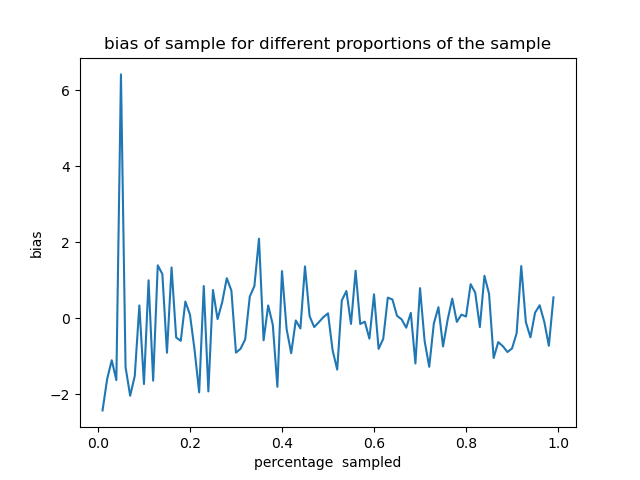
\includegraphics[width=10cm]{/home/buzgalbraith/work/school/spring_2023/probaility-theroy-2-2023/homework/homework_3/immages/Figure_1.png}
    \begin{itemize}
        \item as can be seen from the above plot sample bias goes down as the proportion of the population used in a sample. further it seems like sample bias is stabilizes with a sample that is around 20$\%$ of the population and stops falling
    \end{itemize} 
    \\ 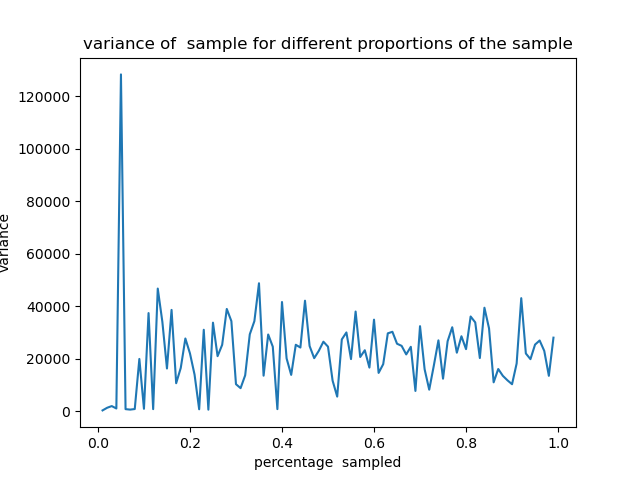
\includegraphics[width=10cm]{/home/buzgalbraith/work/school/spring_2023/probaility-theroy-2-2023/homework/homework_3/immages/Figure_2.png}
        \begin{itemize}
                \item as can be seen from the above plot sample variance goes down as the proportion of the population used in a sample. further it seems like sample variance is stabilizes with a sample that is around 20$\%$ of the population and stops falling
    \end{itemize}
\end{enumerate}


\item Approximate the probability that \textit{ap\_hi} deviates from the corresponding population mean via Monte Carlo simulations, and compare it to the Chebyshev bound that we use to prove the law of large numbers.
\begin{itemize}
\item i was not entirely sure how we were supposed to show this, but here are some figures that i think illustrate the relationship well.
\begin{enumerate}
    \item 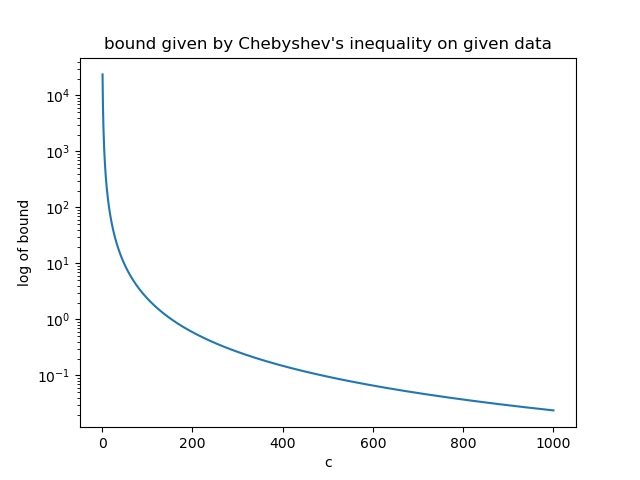
\includegraphics[width=10cm]{/home/buzgalbraith/work/school/spring_2023/probaility-theroy-2-2023/homework/homework_3/immages/Figure_4.png}
    \begin{itemize}
        \item the variance of our data is 23719.178472621654 which is very high. so thus we would need $\epsilon\geq154.01031937055924$ to bound $P(|\Tilde{x}-\mu|\geq \epsilon)\leq 1$
        \item so as can  be seen from this chart and Chebyshev's inequality vies us a very louse bound for this data  
    \end{itemize}
    \item 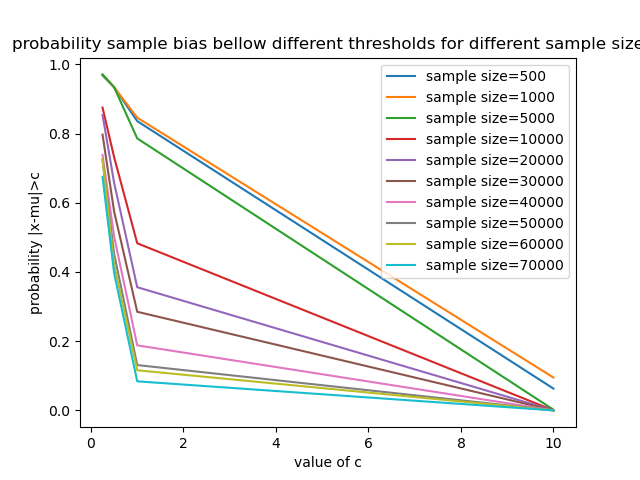
\includegraphics[width=12cm]{/home/buzgalbraith/work/school/spring_2023/probaility-theroy-2-2023/homework/homework_3/immages/Figure_3.png}
    \begin{itemize}
        \item this graph shows the empirical probability calculated using Monte Carlo methods that the sample mean is bellow various values of $\epsilon$ 
        \item each line shows how the path of this likelihood varies for different sample sizes
        \item the real take away of this, is we can establish a frailly tight bound using simulation 
    \end{itemize}
    \item so in conclusion for samples with high variance and a well defined mean, empirical methods can be better used to bound the probability that our estimator will differ from the population parameter more tightly than Chebyshev's inequality 
\end{enumerate}
\end{itemize}
\end{enumerate}
\end{enumerate}
\end{document}
